% This file was created with tikzplotlib v0.10.1.
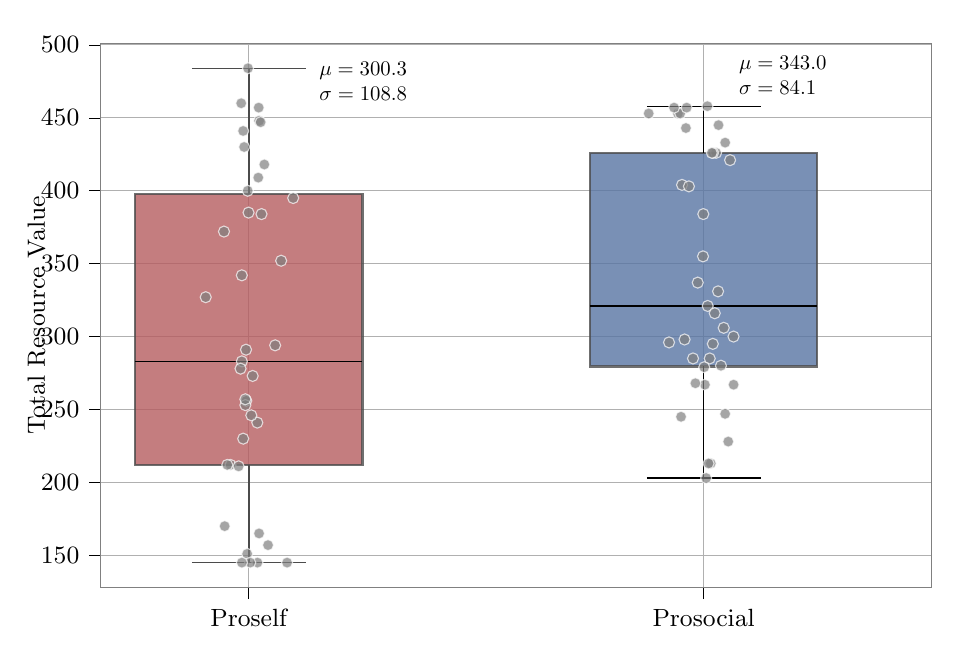
\begin{tikzpicture}[scale= 1]

\definecolor{darkgrey176}{RGB}{176,176,176}
\definecolor{darkslategrey}{RGB}{47,79,79}
\definecolor{darkslategrey75}{RGB}{75,75,75}
\definecolor{grey}{RGB}{128,128,128}
\definecolor{indianred1819295}{RGB}{181,92,95}
\definecolor{steelblue88116163}{RGB}{88,116,163}
\definecolor{grey127}{RGB}{127,127,127}
\begin{axis}[
    width=1\textwidth,    % 增加宽度
    height=0.7\textwidth,   % 保持高度
    axis line style={grey},
    legend cell align={left},
    legend style={
        fill opacity=1,
        draw opacity=1,
        text opacity=1,
        draw=lightgrey204,
        font=\small
    },
    tick align=outside,
    tick pos=left,
    tick label style={font=\small}, % 减小刻度标签文字大小
    unbounded coords=jump,
    x grid style={darkgrey176},
    xmajorgrids,
    xmin=-0.325,
    xmax=1.5,  % 增加右侧空间
    xtick style={color=black},
    xtick={0,1},
    xticklabels={Proself,Prosocial},
    y grid style={darkgrey176},
    ylabel={Total Resource Value},
    ylabel style={
        inner sep=0pt,    % 减少标签和轴的距离
        yshift=-5pt,
        font=\small% 微调标签位置
    },
    ymajorgrids,
    ymin=128.05,
    ymax=500.95,
    ytick style={color=black}
]

\path [draw=darkslategrey75, fill=indianred1819295, opacity=0.8, thick]
(axis cs:-0.25,212)
--(axis cs:0.25,212)
--(axis cs:0.25,397.5)
--(axis cs:-0.25,397.5)
--(axis cs:-0.25,212)
--cycle;
\addplot [thick, darkslategrey75]
table {%
0 212
0 145
};
\addplot [thick, darkslategrey75]
table {%
0 397.5
0 484
};
\addplot [darkslategrey75]
table {%
-0.125 145
0.125 145
};
\addplot [darkslategrey75]
table {%
-0.125 484
0.125 484
};
\path [draw=darkslategrey75, fill=steelblue88116163, opacity=0.8, thick]
(axis cs:0.75,279.5)
--(axis cs:1.25,279.5)
--(axis cs:1.25,426)
--(axis cs:0.75,426)
--(axis cs:0.75,279.5)
--cycle;
\addplot [semithick, black]
table {%
1 279.5
1 203
};
\addplot [semithick, black]
table {%
1 426
1 458
};
\addplot [black]
table {%
0.875 203
1.125 203
};
\addplot [black]
table {%
0.875 458
1.125 458
};
\addplot [semithick, black]
table {%
-0.25 283
0.25 283
};
\addplot [semithick, black]
table {%
0.75 321
1.25 321
};
\addplot [draw=white, fill=grey127, mark=*, only marks, opacity=0.7]
table{%
x  y
-0.0400714931851179 212
-0.0471077322208402 212
-0.00348859589556723 151
-0.00535089710335726 256
0.0188237301177679 241
-0.0528967007198037 170
0.0342792737565218 418
0.0227967510587223 448
0.021889248835996 457
0.0424060017506745 157
0.0226896689679356 165
0.0190811233108301 145
0.0842751337063159 145
0.00328385078573139 145
-0.015058423667463 145
-0.00225422671150385 400
-0.0151309330843346 283
0.0580573976352849 294
-0.007403861239717 253
-0.00746582744592909 257
-0.0222577633297763 211
-0.0945623517165704 327
-0.000459986797348707 385
0.0260911422409645 447
-0.054421902227173 372
0.0209726357676193 409
0.0280668742631608 384
-0.015211997737578 342
0.0977132767945952 395
-0.012148787362295 230
-0.018010351217818 278
0.00865172163974299 273
0.00561699758303698 246
-0.0165485111999984 460
-0.0100909696563266 430
-0.0122865212285328 441
-0.00598001510483728 291
0.0712729100178481 352
-0.001671465968594 484
};
\addplot [draw=white, fill=grey127, mark=*, only marks, opacity=0.7]
table{%
x  y
1.0441367553066 306
1.0027332433394 267
0.95806292071245 298
0.950327774587431 245
0.976652722074529 285
1.01329328712134 285
1.06579537883704 267
1.01558799679811 213
1.00554778845784 203
0.981861072208001 268
1.03799438299505 280
1.00887494972378 321
1.06565853282715 300
1.02432677880316 316
0.986987431934729 337
1.05404842765952 228
0.923907194855337 296
1.00122851638026 279
1.01072624258051 213
1.02014635388555 295
1.03169376989667 331
0.943346312961445 453
0.87918469572047 453
0.948499504536591 453
1.02738130216741 426
1.02066958997992 426
1.05808479915307 421
1.01797718789997 426
0.960991304116238 443
1.00825805416717 458
1.04721016525747 247
0.998592361718987 355
1.03265007319596 445
1.04729862844036 433
0.999219551792941 384
0.952445320354032 404
0.967587585006039 403
0.96264876180953 457
0.934955276115197 457
};

% 调整统计信息的位置和样式
\draw (axis cs:0.15,490) node[
  scale=0.75,
  fill=none,
  draw=none,
  inner sep=1pt,
  anchor=north west,
  text=black,
  align=left
]{\bfseries $\mu = 300.3$\\
$\sigma = 108.8$};

\draw (axis cs:1.07,495) node[
  scale=0.75,
  fill=none,
  draw=none,
  inner sep=1.5pt,
  anchor=north west,
  text=black,
  align=left
]{\bfseries $\mu = 343.0$\\
$\sigma = 84.1$};

\end{axis}
\end{tikzpicture}